\section{CServer\-Instance  Class Reference}
\label{classCServerInstance}\index{CServerInstance@{CServer\-Instance}}
{\tt \#include $<$CServer\-Instance.h$>$}

Inheritance diagram for CServer\-Instance::\begin{figure}[H]
\begin{center}
\leavevmode
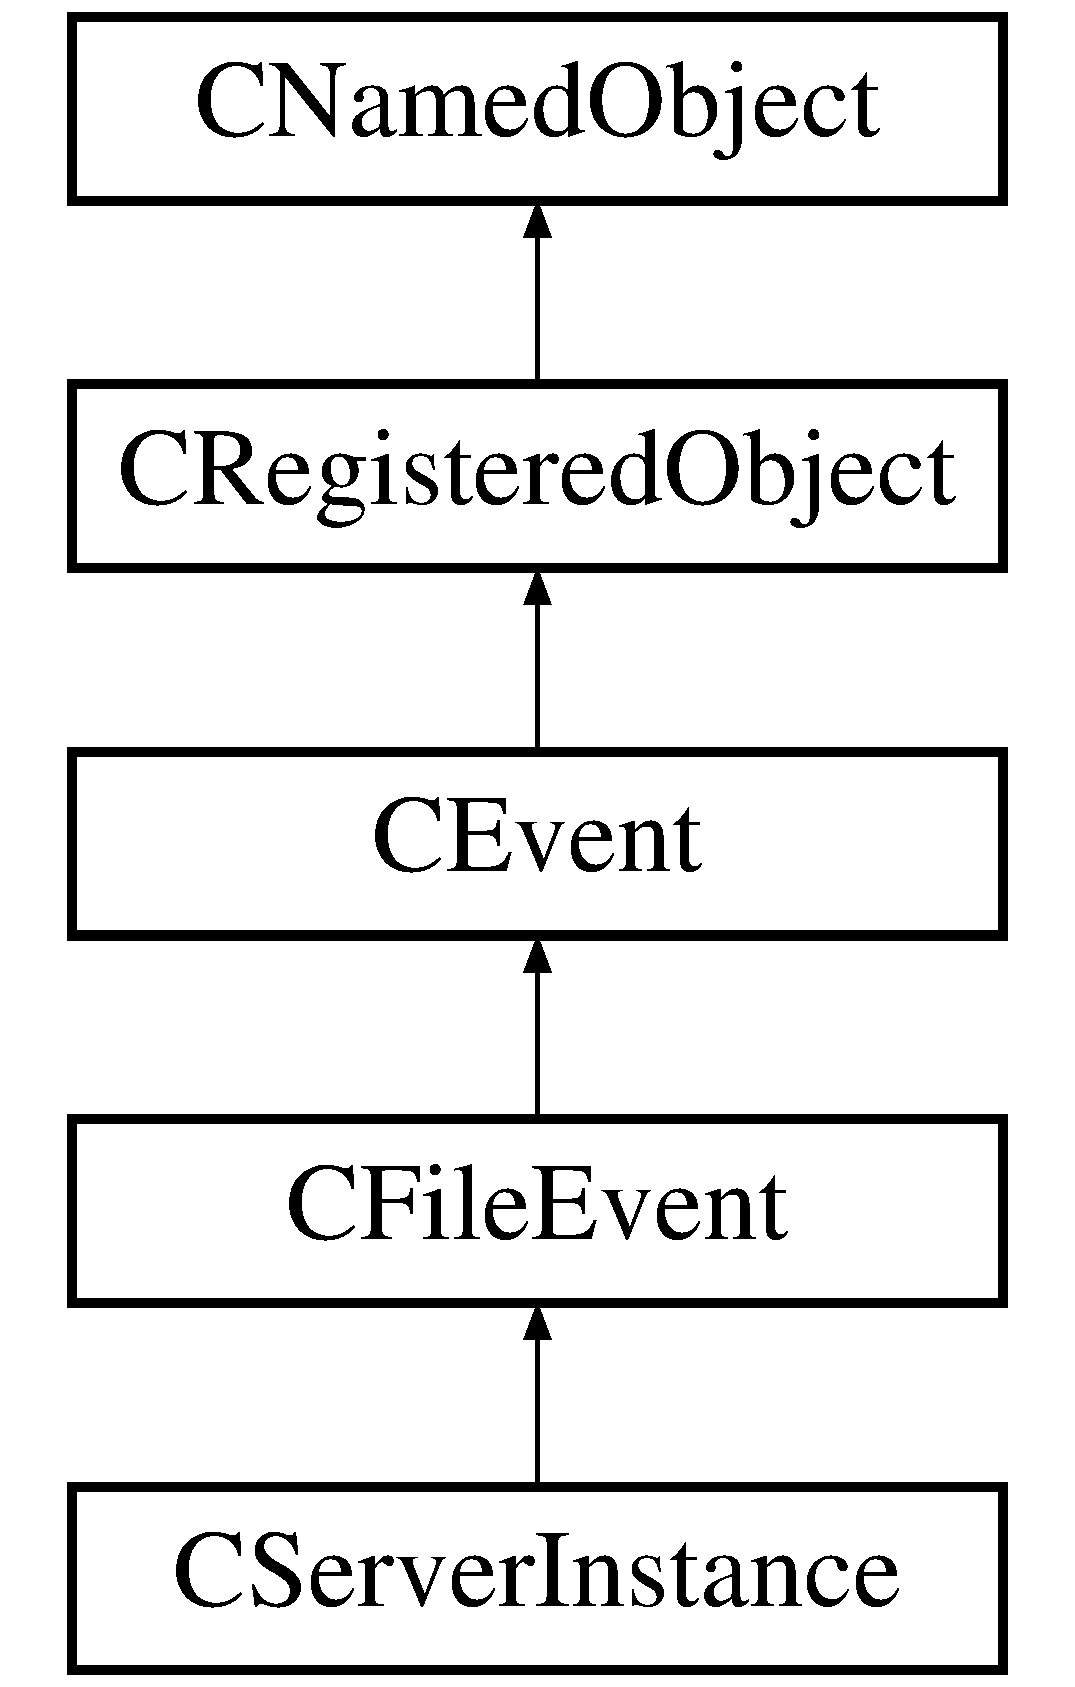
\includegraphics[height=5cm]{classCServerInstance}
\end{center}
\end{figure}
\subsection*{Public Methods}
\begin{CompactItemize}
\item 
{\bf CServer\-Instance} ({\bf CSocket} $\ast$p\-Socket, bool f\-Delete\-Socket=true)
\item 
{\bf CServer\-Instance} (const char $\ast$p\-Name, {\bf CSocket} $\ast$p\-Socket, bool f\-Delete\-Socket=true)
\item 
{\bf CServer\-Instance} (const string \&r\-Name, {\bf CSocket} $\ast$p\-Socket, bool f\-Delete\-Socket=true)
\item 
{\bf $\sim$CServer\-Instance} ()
\item 
{\bf CSocket} $\ast$ {\bf get\-Socket} ()
\item 
bool {\bf get\-Delete\-Flag} () const
\item 
string {\bf get\-Peername} () const
\item 
unsigned short {\bf get\-Peer\-Port} () const
\item 
virtual void {\bf On\-Readable} (istream \&r\-Stream)
\item 
virtual void {\bf On\-Request} ({\bf CSocket} $\ast$p\-Connection)
\item 
void {\bf Shutdown} ()
\item 
virtual string {\bf Describe\-Self} ()
\end{CompactItemize}
\subsection*{Protected Methods}
\begin{CompactItemize}
\item 
void {\bf set\-Socket} ({\bf CSocket} $\ast$sock)
\item 
void {\bf set\-Del\-Flag} (bool flag)
\end{CompactItemize}
\subsection*{Private Methods}
\begin{CompactItemize}
\item 
{\bf CServer\-Instance} (const CServer\-Instance \&rhs)
\item 
CServer\-Instance \& {\bf operator=} (const CServer\-Instance \&rhs)
\item 
int {\bf operator==} (const CServer\-Instance \&rhs)
\end{CompactItemize}
\subsection*{Private Attributes}
\begin{CompactItemize}
\item 
{\bf CSocket} $\ast$ {\bf m\_\-p\-Peer}
\begin{CompactList}\small\item\em Pointer to peer socket.\item\end{CompactList}\item 
bool {\bf m\_\-f\-Delete\-Socket}
\begin{CompactList}\small\item\em True if destructor deletes socket.\item\end{CompactList}\end{CompactItemize}


\subsection{Detailed Description}
Encapsulates the funtionality of a `simple' Tcp/Ip server instance. Simpler tcp/ip server instances are connections with a client over a socket which operate in the simple::\begin{CompactItemize}
\item 
Accept a request from the client.\item 
Respond to those requests mode.\end{CompactItemize}
This class is a subclass of the {\bf CFile\-Event} {\rm (p.\,\pageref{classCFileEvent})} class... On\-Readable is overridden by this class, the user, should in turn override this class and override {\bf On\-Request}() {\rm (p.\,\pageref{classCServerInstance_a9})}. {\bf On\-Request}() {\rm (p.\,\pageref{classCServerInstance_a9})} entered with the application serialization mutex held, and therefore can perform any function which requires global syncrhonization. 



Definition at line 321 of file CServer\-Instance.h.

\subsection{Constructor \& Destructor Documentation}
\index{CServerInstance@{CServer\-Instance}!CServerInstance@{CServerInstance}}
\index{CServerInstance@{CServerInstance}!CServerInstance@{CServer\-Instance}}
\subsubsection{\setlength{\rightskip}{0pt plus 5cm}CServer\-Instance::CServer\-Instance ({\bf CSocket} $\ast$ {\em p\-Socket}, bool {\em f\-Delete\-Socket} = true)}\label{classCServerInstance_a0}


Construct an anonymous server instance:\begin{Desc}
\item[Parameters: ]\par
\begin{description}
\item[{\em 
p\-Socket}]- Pointer to the socket open to the client. \item[{\em 
f\-Delete\-Socket}]- true if the destructor should delete the socket. \end{description}
\end{Desc}


Definition at line 300 of file CServer\-Instance.cpp.\index{CServerInstance@{CServer\-Instance}!CServerInstance@{CServerInstance}}
\index{CServerInstance@{CServerInstance}!CServerInstance@{CServer\-Instance}}
\subsubsection{\setlength{\rightskip}{0pt plus 5cm}CServer\-Instance::CServer\-Instance (const char $\ast$ {\em p\-Name}, {\bf CSocket} $\ast$ {\em p\-Socket}, bool {\em f\-Delete\-Socket} = true)}\label{classCServerInstance_a1}


Construct a server instance whose name comes from a char$\ast$ string.\begin{Desc}
\item[Parameters: ]\par
\begin{description}
\item[{\em 
p\-Name}]- Name to give to the instance (const char$\ast$) [in] \item[{\em 
p\-Socket}]- Socket open on peer. ({\bf CSocket} {\rm (p.\,\pageref{classCSocket})}$\ast$ ) [in] \item[{\em 
f\-Delete\-Socket}]- true to delete sock on destruct (bool) [in = true] \end{description}
\end{Desc}


Definition at line 314 of file CServer\-Instance.cpp.\index{CServerInstance@{CServer\-Instance}!CServerInstance@{CServerInstance}}
\index{CServerInstance@{CServerInstance}!CServerInstance@{CServer\-Instance}}
\subsubsection{\setlength{\rightskip}{0pt plus 5cm}CServer\-Instance::CServer\-Instance (const string \& {\em r\-Name}, {\bf CSocket} $\ast$ {\em p\-Socket}, bool {\em f\-Delete\-Socket} = true)}\label{classCServerInstance_a2}


Construct a server instance whose name comes from a string\& string.\begin{Desc}
\item[Parameters: ]\par
\begin{description}
\item[{\em 
r\-Name}]- Name to give to the instance (const string\& [in]). \item[{\em 
p\-Socket-}]Socket already open on peer ({\bf CSocket} {\rm (p.\,\pageref{classCSocket})}$\ast$ [in]). \item[{\em 
f\-Delete\-Socket}]- true to delete sock on destruction. (bool [in] = true). \end{description}
\end{Desc}


Definition at line 328 of file CServer\-Instance.cpp.\index{CServerInstance@{CServer\-Instance}!~CServerInstance@{$\sim$CServerInstance}}
\index{~CServerInstance@{$\sim$CServerInstance}!CServerInstance@{CServer\-Instance}}
\subsubsection{\setlength{\rightskip}{0pt plus 5cm}CServer\-Instance::$\sim$CServer\-Instance ()}\label{classCServerInstance_a3}


The destructor just deletes m\_\-p\-Peer if m\_\-f\-Delete\-Socket is true. 

Definition at line 338 of file CServer\-Instance.cpp.

References CSocket::Connected, CSocket::get\-State(), m\_\-p\-Peer, and CSocket::Shutdown().\index{CServerInstance@{CServer\-Instance}!CServerInstance@{CServerInstance}}
\index{CServerInstance@{CServerInstance}!CServerInstance@{CServer\-Instance}}
\subsubsection{\setlength{\rightskip}{0pt plus 5cm}CServer\-Instance::CServer\-Instance (const CServer\-Instance \& {\em rhs})\hspace{0.3cm}{\tt  [private]}}\label{classCServerInstance_c0}




\subsection{Member Function Documentation}
\index{CServerInstance@{CServer\-Instance}!DescribeSelf@{DescribeSelf}}
\index{DescribeSelf@{DescribeSelf}!CServerInstance@{CServer\-Instance}}
\subsubsection{\setlength{\rightskip}{0pt plus 5cm}string CServer\-Instance::Describe\-Self ()\hspace{0.3cm}{\tt  [virtual]}}\label{classCServerInstance_a11}


Describe this textually. 

Reimplemented from {\bf CFile\-Event} {\rm (p.\,\pageref{classCFileEvent_a19})}.

Definition at line 447 of file CServer\-Instance.cpp.

References CEvent::Describe\-Self(), CSocket::get\-Socket\-Fd(), CSocket::get\-State(), m\_\-f\-Delete\-Socket, m\_\-p\-Peer, and CSocket::State\-Name().\index{CServerInstance@{CServer\-Instance}!getDeleteFlag@{getDeleteFlag}}
\index{getDeleteFlag@{getDeleteFlag}!CServerInstance@{CServer\-Instance}}
\subsubsection{\setlength{\rightskip}{0pt plus 5cm}bool CServer\-Instance::get\-Delete\-Flag () const\hspace{0.3cm}{\tt  [inline]}}\label{classCServerInstance_a5}




Definition at line 349 of file CServer\-Instance.h.

References m\_\-f\-Delete\-Socket.\index{CServerInstance@{CServer\-Instance}!getPeername@{getPeername}}
\index{getPeername@{getPeername}!CServerInstance@{CServer\-Instance}}
\subsubsection{\setlength{\rightskip}{0pt plus 5cm}string CServer\-Instance::get\-Peername () const}\label{classCServerInstance_a6}


Determines the node to which this socket is connected.\begin{Desc}
\item[Return values: ]\par
\begin{description}
\item[{\em 
string\&}]The name of the peer to which this socket is connected. if the peer has a dns entry the name of the peer is returned, otherwise the IP address is converted to dotted string form and returned. See {\bf CSocket::get\-Peer}() {\rm (p.\,\pageref{classCSocket_a13})}\end{description}
\end{Desc}
\begin{Desc}
\item[Note: ]\par
Can throw any exception thrown by {\bf CSocket::get\-Peer}() {\rm (p.\,\pageref{classCSocket_a13})} \end{Desc}


Definition at line 361 of file CServer\-Instance.cpp.

References CSocket::get\-Peer(), and m\_\-p\-Peer.\index{CServerInstance@{CServer\-Instance}!getPeerPort@{getPeerPort}}
\index{getPeerPort@{getPeerPort}!CServerInstance@{CServer\-Instance}}
\subsubsection{\setlength{\rightskip}{0pt plus 5cm}unsigned short CServer\-Instance::get\-Peer\-Port () const}\label{classCServerInstance_a7}


Determines the port to which the socket is connected on the peer.\begin{Desc}
\item[Return values: ]\par
\begin{description}
\item[{\em 
int}]The port number assigned to this socket.\end{description}
\end{Desc}
\begin{Desc}
\item[Note: ]\par
Can throw any exception thrown by {\bf CSocket::get\-Peer}() {\rm (p.\,\pageref{classCSocket_a13})} \end{Desc}


Definition at line 380 of file CServer\-Instance.cpp.

References CSocket::get\-Peer(), and m\_\-p\-Peer.\index{CServerInstance@{CServer\-Instance}!getSocket@{getSocket}}
\index{getSocket@{getSocket}!CServerInstance@{CServer\-Instance}}
\subsubsection{\setlength{\rightskip}{0pt plus 5cm}{\bf CSocket}$\ast$ CServer\-Instance::get\-Socket ()\hspace{0.3cm}{\tt  [inline]}}\label{classCServerInstance_a4}




Definition at line 346 of file CServer\-Instance.h.\index{CServerInstance@{CServer\-Instance}!OnReadable@{OnReadable}}
\index{OnReadable@{OnReadable}!CServerInstance@{CServer\-Instance}}
\subsubsection{\setlength{\rightskip}{0pt plus 5cm}void CServer\-Instance::On\-Readable (istream \& {\em r\-Input})\hspace{0.3cm}{\tt  [virtual]}}\label{classCServerInstance_a8}


Called when the socket becomes readable. We get the socket and pass that to On\-Request which is what the user is supposed to override and embed application functionality in.\begin{Desc}
\item[Parameters: ]\par
\begin{description}
\item[{\em 
r\-Input}]- Stream open on the socket (istream\& [in-out])\end{description}
\end{Desc}
\begin{Desc}
\item[Note: ]\par
DO NOT OVERRIDE THIS \end{Desc}


Reimplemented from {\bf CFile\-Event} {\rm (p.\,\pageref{classCFileEvent_a15})}.

Definition at line 402 of file CServer\-Instance.cpp.

References m\_\-p\-Peer, On\-Request(), and Shutdown().\index{CServerInstance@{CServer\-Instance}!OnRequest@{OnRequest}}
\index{OnRequest@{OnRequest}!CServerInstance@{CServer\-Instance}}
\subsubsection{\setlength{\rightskip}{0pt plus 5cm}void CServer\-Instance::On\-Request ({\bf CSocket} $\ast$ {\em p\-Connection})\hspace{0.3cm}{\tt  [virtual]}}\label{classCServerInstance_a9}


Called when the client has a request of the server. The application has overridden this member in its derived class.\begin{Desc}
\item[Parameters: ]\par
\begin{description}
\item[{\em 
p\-Connection}]- Socket open to the peer ({\bf CSocket} {\rm (p.\,\pageref{classCSocket})}$\ast$ [in-out]). \end{description}
\end{Desc}


Definition at line 418 of file CServer\-Instance.cpp.

Referenced by On\-Readable().\index{CServerInstance@{CServer\-Instance}!operator=@{operator=}}
\index{operator=@{operator=}!CServerInstance@{CServer\-Instance}}
\subsubsection{\setlength{\rightskip}{0pt plus 5cm}CServer\-Instance\& CServer\-Instance::operator= (const CServer\-Instance \& {\em rhs})\hspace{0.3cm}{\tt  [private]}}\label{classCServerInstance_c1}


\index{CServerInstance@{CServer\-Instance}!operator==@{operator==}}
\index{operator==@{operator==}!CServerInstance@{CServer\-Instance}}
\subsubsection{\setlength{\rightskip}{0pt plus 5cm}int CServer\-Instance::operator== (const CServer\-Instance \& {\em rhs})\hspace{0.3cm}{\tt  [private]}}\label{classCServerInstance_c2}


\index{CServerInstance@{CServer\-Instance}!setDelFlag@{setDelFlag}}
\index{setDelFlag@{setDelFlag}!CServerInstance@{CServer\-Instance}}
\subsubsection{\setlength{\rightskip}{0pt plus 5cm}void CServer\-Instance::set\-Del\-Flag (bool {\em flag})\hspace{0.3cm}{\tt  [inline, protected]}}\label{classCServerInstance_b1}




Definition at line 361 of file CServer\-Instance.h.

References m\_\-f\-Delete\-Socket.\index{CServerInstance@{CServer\-Instance}!setSocket@{setSocket}}
\index{setSocket@{setSocket}!CServerInstance@{CServer\-Instance}}
\subsubsection{\setlength{\rightskip}{0pt plus 5cm}void CServer\-Instance::set\-Socket ({\bf CSocket} $\ast$ {\em sock})\hspace{0.3cm}{\tt  [inline, protected]}}\label{classCServerInstance_b0}




Definition at line 358 of file CServer\-Instance.h.\index{CServerInstance@{CServer\-Instance}!Shutdown@{Shutdown}}
\index{Shutdown@{Shutdown}!CServerInstance@{CServer\-Instance}}
\subsubsection{\setlength{\rightskip}{0pt plus 5cm}void CServer\-Instance::Shutdown ()}\label{classCServerInstance_a10}


Called when we want to shutdown the server we must:\begin{enumerate}
\item 
Remove all fd monitoring.\item 
Clear the enable flag.\item 
Shutdown the socket.\end{enumerate}
It's someone else's responsibility to reap these threads and delete the objects. 

Definition at line 434 of file CServer\-Instance.cpp.

References CSocket::Connected, CSocket::get\-State(), m\_\-p\-Peer, CFile\-Event::Monitor\-Readable(), CEvent::set\-Enable(), and CSocket::Shutdown().

Referenced by On\-Readable().

\subsection{Member Data Documentation}
\index{CServerInstance@{CServer\-Instance}!m_fDeleteSocket@{m\_\-fDeleteSocket}}
\index{m_fDeleteSocket@{m\_\-fDeleteSocket}!CServerInstance@{CServer\-Instance}}
\subsubsection{\setlength{\rightskip}{0pt plus 5cm}bool CServer\-Instance::m\_\-f\-Delete\-Socket\hspace{0.3cm}{\tt  [private]}}\label{classCServerInstance_o1}


True if destructor deletes socket.



Definition at line 325 of file CServer\-Instance.h.

Referenced by Describe\-Self(), get\-Delete\-Flag(), and set\-Del\-Flag().\index{CServerInstance@{CServer\-Instance}!m_pPeer@{m\_\-pPeer}}
\index{m_pPeer@{m\_\-pPeer}!CServerInstance@{CServer\-Instance}}
\subsubsection{\setlength{\rightskip}{0pt plus 5cm}{\bf CSocket}$\ast$ CServer\-Instance::m\_\-p\-Peer\hspace{0.3cm}{\tt  [private]}}\label{classCServerInstance_o0}


Pointer to peer socket.



Definition at line 324 of file CServer\-Instance.h.

Referenced by Describe\-Self(), get\-Peername(), get\-Peer\-Port(), On\-Readable(), Shutdown(), and $\sim$CServer\-Instance().

The documentation for this class was generated from the following files:\begin{CompactItemize}
\item 
{\bf CServer\-Instance.h}\item 
{\bf CServer\-Instance.cpp}\end{CompactItemize}
